\documentclass[11pt]{article}
\usepackage[utf8]{inputenc}
\usepackage{amsmath,amssymb,amsthm,amsfonts}
\usepackage{graphicx}
\usepackage{booktabs}
\usepackage{url}
\usepackage{hyperref}
\usepackage{caption}
\usepackage{subcaption}

\usepackage{algorithm}
\usepackage{algpseudocode}

\usepackage{tikz}
\usetikzlibrary{matrix,fit,positioning}


\title{Cool \& Cruel++: Hybrid Secret Recovery of Binary Sparse LWE Secrets}
\author{Your Name \\ \small{Your University / Lab of Cryptography}}
\date{\today}

\begin{document}
\maketitle

\begin{abstract}
Sparse binary LWE secrets are widely used in homomorphic encryption for efficiency, but recent work highlights potential vulnerabilities. This paper provides a comprehensive overview of the ``Cool and Cruel'' attack---a partial-lattice-reduction-based method that separates LWE secrets into a ``cruel'' (unreduced) portion requiring brute-force enumeration and a ``cool'' (reduced) portion recoverable via fast statistical tests. We detail the core ideas, including partial reduction trade-offs, variance-based distinguishers, GPU-accelerated enumeration, and the extension to 2-power cyclotomic Ring-LWE. The presented results illustrate that for certain parameter sets, this approach significantly reduces memory requirements compared to older meet-in-the-middle attacks, while achieving real-world feasibility even for dimensions $n \leq 1024$. We conclude by discussing the implications for cryptographic scheme designers and paving the way for further study on mitigating such attacks.
\end{abstract}

\begin{figure}[ht]
  \centering
  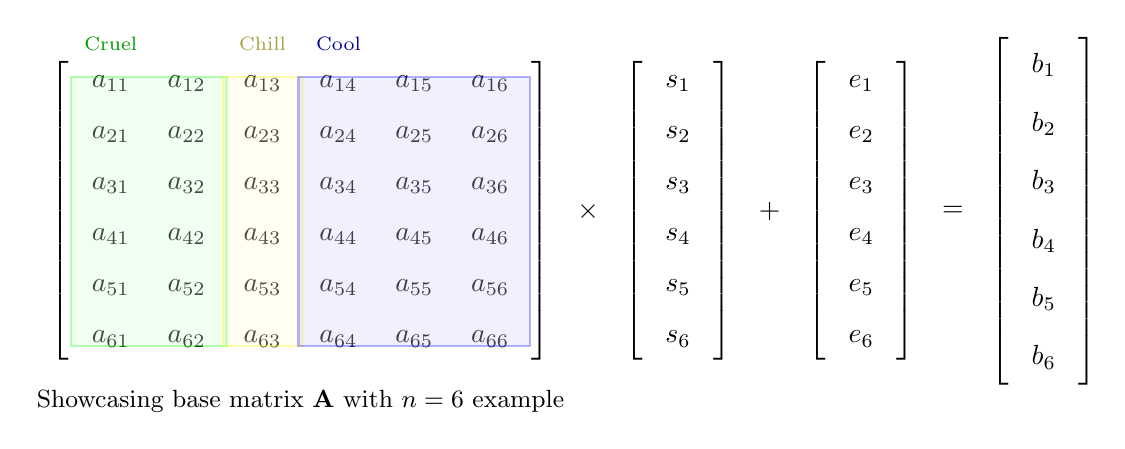
\begin{tikzpicture}[>=stealth, node distance=1.2cm]
  
  %--- Matrix A with coefficients a_ij
  \matrix[matrix of math nodes,
          row sep=0.6em,
          column sep=0.7em,
          left delimiter={[},
          right delimiter={]},
          nodes={minimum size=1em, anchor=center}
          ] (A) {
    a_{11} & a_{12} & a_{13} & a_{14} & a_{15} & a_{16} \\
    a_{21} & a_{22} & a_{23} & a_{24} & a_{25} & a_{26} \\
    a_{31} & a_{32} & a_{33} & a_{34} & a_{35} & a_{36} \\
    a_{41} & a_{42} & a_{43} & a_{44} & a_{45} & a_{46} \\
    a_{51} & a_{52} & a_{53} & a_{54} & a_{55} & a_{56} \\
    a_{61} & a_{62} & a_{63} & a_{64} & a_{65} & a_{66} \\
  };
  
  %--- Highlighting columns for Cruel, Chill, and Cool
  \draw[thick, green, opacity=0.3, fill=green!20]
    ([xshift=-4pt,yshift=-4pt]A-1-1.north west) 
    rectangle ([xshift=4pt,yshift=4pt]A-6-2.south east);
  \node[above=2pt,green!60!black] at (A-1-1.north) {\scriptsize Cruel};
  
  \draw[thick, yellow, opacity=0.3, fill=yellow!20]
    ([xshift=-4pt,yshift=-4pt]A-1-3.north west)
    rectangle ([xshift=4pt,yshift=4pt]A-6-3.south east);
  \node[above=2pt,yellow!60!black] at (A-1-3.north) {\scriptsize Chill};
  
  \draw[thick, blue, opacity=0.3, fill=blue!20]
    ([xshift=-4pt,yshift=-4pt]A-1-4.north west)
    rectangle ([xshift=4pt,yshift=4pt]A-6-6.south east);
  \node[above=2pt,blue!60!black] at (A-1-4.north) {\scriptsize Cool};
  
  \node[right=0.5cm of A] (miltiply) {$\times$};

  %--- Secret vector s
  \matrix[matrix of math nodes,
          row sep=0.6em,
          column sep=0.7em,
          left delimiter={[},
          right delimiter={]},
          nodes={minimum size=1em, anchor=center},
          right=1.5cm of A
          ] (s) {
    s_1 \\
    s_2 \\
    s_3 \\
    s_4 \\
    s_5 \\
    s_6 \\
  };

  %--- Plus Error term
  \node[right=0.5cm of s] (plus) {$+$};
  
  \matrix[matrix of math nodes,
          row sep=0.6em,
          column sep=0.7em,
          left delimiter={[},
          right delimiter={]},
          nodes={minimum size=1em, anchor=center},
          right=0.5cm of plus
          ] (e) {
    e_1 \\
    e_2 \\
    e_3 \\
    e_4 \\
    e_5 \\
    e_6 \\
  };

  %--- Equals sign
  \node[right=0.5cm of e] (eq) {$=$};

  %--- Resulting vector b
  \matrix[matrix of math nodes,
          row sep=0.6em,
          column sep=0.7em,
          left delimiter={[},
          right delimiter={]},
          nodes={minimum size=1em, anchor=center},
          right=0.5cm of eq
          ] (b) {
    b_1 \\
    b_2 \\
    b_3 \\
    b_4 \\
    b_5 \\
    b_6 \\
  };

  %--- Caption
  \node[below=5pt of A] {\small Showcasing base matrix $\mathbf{A}$ with $n=6$ example};
  
  \end{tikzpicture}
  \caption{Ring-LWE matrix in skew-circulant form, split into \textbf{Cruel} (green), \textbf{Chill} (yellow), and \textbf{Cool} (blue) column regions. Multiplying by secret $\mathbf{s}$ and adding error $\mathbf{e}$ produces $\mathbf{b}$.}
  \label{fig:rlwe_circ_cool_chill_cruel}
\end{figure}


\begin{figure}[ht]

  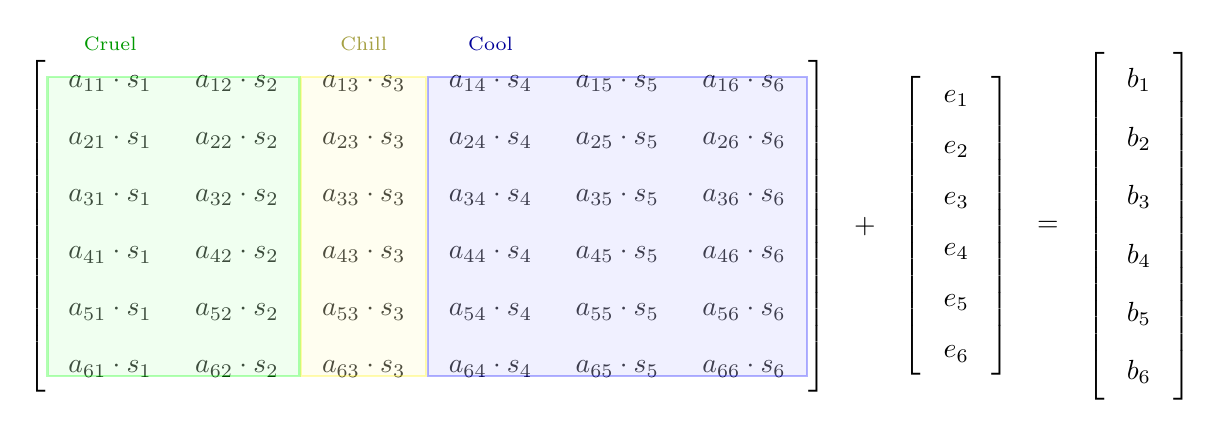
\begin{tikzpicture}[>=stealth, distance=1.2cm]
  
  %--- Matrix A with explicit multiplications
  \matrix[matrix of math nodes,
          row sep=0.8em,
          column sep=0.9em,
          left delimiter={[},
          right delimiter={]},
          nodes={minimum size=1em, anchor=center}
    ] (A) {
    a_{11} \cdot s_1 & a_{12} \cdot s_2 & a_{13} \cdot s_3 & a_{14} \cdot s_4 & a_{15} \cdot s_5 & a_{16} \cdot s_6 \\
    a_{21} \cdot s_1 & a_{22} \cdot s_2 & a_{23} \cdot s_3 & a_{24} \cdot s_4 & a_{25} \cdot s_5 & a_{26} \cdot s_6 \\
    a_{31} \cdot s_1 & a_{32} \cdot s_2 & a_{33} \cdot s_3 & a_{34} \cdot s_4 & a_{35} \cdot s_5 & a_{36} \cdot s_6 \\
    a_{41} \cdot s_1 & a_{42} \cdot s_2 & a_{43} \cdot s_3 & a_{44} \cdot s_4 & a_{45} \cdot s_5 & a_{46} \cdot s_6 \\
    a_{51} \cdot s_1 & a_{52} \cdot s_2 & a_{53} \cdot s_3 & a_{54} \cdot s_4 & a_{55} \cdot s_5 & a_{56} \cdot s_6 \\
    a_{61} \cdot s_1 & a_{62} \cdot s_2 & a_{63} \cdot s_3 & a_{64} \cdot s_4 & a_{65} \cdot s_5 & a_{66} \cdot s_6 \\
  };

    %--- Highlighting columns for Cruel, Chill, and Cool
    \draw[thick, green, opacity=0.3, fill=green!20]
    ([xshift=-4pt,yshift=-4pt]A-1-1.north west) 
    rectangle ([xshift=4pt,yshift=4pt]A-6-2.south east);
  \node[above=2pt,green!60!black] at (A-1-1.north) {\scriptsize Cruel};
  
  \draw[thick, yellow, opacity=0.3, fill=yellow!20]
    ([xshift=-4pt,yshift=-4pt]A-1-3.north west)
    rectangle ([xshift=4pt,yshift=4pt]A-6-3.south east);
  \node[above=2pt,yellow!60!black] at (A-1-3.north) {\scriptsize Chill};
  
  \draw[thick, blue, opacity=0.3, fill=blue!20]
    ([xshift=-4pt,yshift=-4pt]A-1-4.north west)
    rectangle ([xshift=4pt,yshift=4pt]A-6-6.south east);
  \node[above=2pt,blue!60!black] at (A-1-4.north) {\scriptsize Cool};

   %--- Plus Error term
   \node[right=0.5cm of A] (plus) {$+$};
  
   \matrix[matrix of math nodes,
           row sep=0.6em,
           column sep=0.7em,
           left delimiter={[},
           right delimiter={]},
           nodes={minimum size=1em, anchor=center},
           right=0.5cm of plus
           ] (e) {
     e_1 \\
     e_2 \\
     e_3 \\
     e_4 \\
     e_5 \\
     e_6 \\
   };
 
   %--- Equals sign
   \node[right=0.5cm of e] (eq) {$=$};
 
   %--- Resulting vector b
   \matrix[matrix of math nodes,
           row sep=0.6em,
           column sep=0.7em,
           left delimiter={[},
           right delimiter={]},
           nodes={minimum size=1em, anchor=center},
           right=0.5cm of eq
           ] (b) {
     b_1 \\
     b_2 \\
     b_3 \\
     b_4 \\
     b_5 \\
     b_6 \\
   };
  
  \end{tikzpicture}
  \caption{Element-wise multiplication of matrix $\mathbf{A}$ with secret $\mathbf{s}$, highlighting Cruel, Chill, and Cool regions.}
  \label{fig:rlwe_matrix_elementwise}
\end{figure}


\begin{frame}{Conventional vs. New Approach: Matrix Schematic}

  \begin{figure}[ht]
      \centering
      %------------------
      % (A) Two-Zone Figure
      %------------------
      \begin{subfigure}[b]{0.45\textwidth}
          \centering
          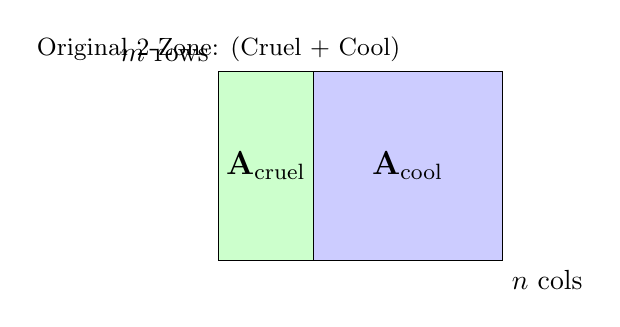
\begin{tikzpicture}[scale=0.8]
            % Draw a matrix shape
            \draw[fill=green!20] (0,0) rectangle (1.5,3) node[midway]{\large $\mathbf{A}_{\mathrm{cruel}}$};
            \draw[fill=blue!20] (1.5,0) rectangle (4.5,3) node[midway]{\large $\mathbf{A}_{\mathrm{cool}}$};
  
            % Axis or dimension labels:
            \draw (0,3) node[above left] {$m$ rows};
            \draw (4.5,0) node[below right] {$n$ cols};
            \draw (0,3) node[above] {\small Original 2-Zone: (Cruel + Cool)};
          \end{tikzpicture}
          \caption{Old Approach: 2-Zone Cruel + Cool}
      \end{subfigure}
      \hfill
      %------------------
      % (B) Three-Zone Figure
      %------------------
      \begin{subfigure}[b]{0.45\textwidth}
          \centering
          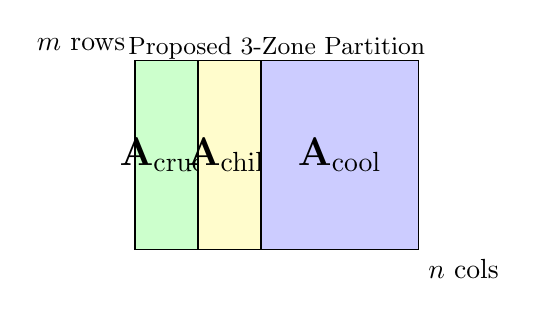
\begin{tikzpicture}[scale=0.8]
            % cruel region
            \draw[fill=green!20] (0,0) rectangle (1.0,3) node[midway] {};
            \node at (0.5,1.5){\Large $\mathbf{A}_{\mathrm{cruel}}$};
  
            % chill region
            \draw[fill=yellow!20] (1.0,0) rectangle (2.0,3) node[midway] {};
            \node at (1.5,1.5){\Large $\mathbf{A}_{\mathrm{chill}}$};
  
            % cool region
            \draw[fill=blue!20] (2.0,0) rectangle (4.5,3) node[midway] {};
            \node at (3.25,1.5){\Large $\mathbf{A}_{\mathrm{cool}}$};
  
            \draw (0,3) node[above left] {$m$ rows};
            \draw (4.5,0) node[below right] {$n$ cols};
  
            \node at (2.25,3.2){\small Proposed 3-Zone Partition};
          \end{tikzpicture}
          \caption{New Approach: 3-Zone (Cruel + Chill + Cool)}
      \end{subfigure}
  
      \caption{\small Schematic: splitting columns of the partially reduced matrix $\mathbf{A}$ into different variance zones.}
  \end{figure}
  \end{frame}
  
  \begin{frame}[fragile]{Proposed Attack: Cool, Chill, and Cruel}

    \small
    \textbf{Assumptions:}
    \begin{itemize}
      \item We already performed partial lattice reduction, so $\mathbf{A}$ has columns with varying std.\ dev.\ $\sigma_j$.
      \item Thresholds $\{T_c, T_h\}$ define which columns are cruel, chill, or cool.
    \end{itemize}
    
    \begin{algorithmic}
    \Procedure{Attack3Zones}{$\mathbf{A},\,\mathbf{b},\,q$}
      \State $(\mathcal{I}_{\mathrm{cruel}},\mathcal{I}_{\mathrm{chill}},\mathcal{I}_{\mathrm{cool}}) \gets \text{ClassifyColumns}(\mathbf{A},T_c,T_h)$
      \State $\mathbf{s}_{\mathrm{cruel}} \gets \mathrm{BruteForceCruel}(\mathbf{A}_{*,\mathcal{I}_{\mathrm{cruel}}}, \mathbf{b})$
      \State $\mathrm{cruel\_ones} \gets \mathrm{HW}(\mathbf{s}_{\mathrm{cruel}})$
    
      \Comment Probabilistic ranking in $\mathcal{I}_{\mathrm{chill}}$
      \State $p_j \gets \mathrm{EstimateProb}(j,\mathbf{A},\mathbf{s}_{\mathrm{cruel}})$ for $j \in \mathcal{I}_{\mathrm{chill}}$
      \State $k = h - \mathrm{cruel\_ones}$  \Comment number of remaining 1-bits
      \State $\mathbf{s}_{\mathrm{chill}} \gets \mathrm{RankAndAssign}(p_j,\;k)$
    
      \Comment Greedy approach for $\mathcal{I}_{\mathrm{cool}}$
      \State $\mathbf{s}_{\mathrm{cool}} \gets \mathrm{GreedyFlip}(\mathbf{A},\mathbf{b},\mathbf{s}_{\mathrm{cruel}},\mathbf{s}_{\mathrm{chill}})$
    
      \Comment Check residual; if not correct, refine $\mathbf{s}_{\mathrm{chill}}$ via local flips
      \State $\mathrm{RefineChill}(\mathbf{A},\mathbf{b},\mathbf{s}_{\mathrm{cruel}},\mathbf{s}_{\mathrm{chill}},\mathbf{s}_{\mathrm{cool}})$
    
      \State \textbf{return} $(\mathbf{s}_{\mathrm{cruel}},\mathbf{s}_{\mathrm{chill}},\mathbf{s}_{\mathrm{cool}})$
    \EndProcedure
    \end{algorithmic}
    
    
    \textbf{Note:}
    - \textproc{EstimateProb} might rely on column variance or partial distribution checks.
    - \textproc{RankAndAssign} picks the top $k$ columns in $\mathcal{I}_{\mathrm{chill}}$ to be 1.
    - \textproc{RefineChill} tries local flips if the final test fails.
    \end{frame}
\section{Introduction}
\label{sec:intro}
Learning With Errors (LWE) has become a cornerstone of post-quantum cryptography and homomorphic encryption (HE). Under standard parameter choices, LWE is believed to be secure even against quantum adversaries. However, many real systems adopt \emph{sparse} secrets (e.g., in $\{0,1\}^n$ with low Hamming weight) to improve efficiency. Such specialized parameter choices can inadvertently introduce vulnerabilities.

This paper focuses on a new statistical attack---the \emph{Cool and Cruel} bit recovery strategy---which shows that partial lattice reduction may separate the LWE instance into a \emph{cruel} portion (retaining high variance) and a \emph{cool} portion (reduced variance). By combining GPU-accelerated enumeration for cruel bits with simple statistical recovery for cool bits, one can break sparse LWE instances more efficiently than older memory-intensive meet-in-the-middle attacks.

\subsection{Previous Work}
\label{sec:previous}
\paragraph{Sparse LWE Attacks.}
Several primal or dual attacks on LWE~\cite{regev,bkz2,flatter} rely on full-dimension lattice reduction. Hybrid meet-in-the-middle approaches (e.g., \cite{ref_mitm}) attempt to guess partial secrets and reduce a lower-dimensional problem. Such methods often demand large memory. Recent approaches, such as SALSA \cite{salsa}, also incorporate machine learning and extensive data sub-sampling.

\paragraph{Distinguishing from Uniform.}
Identifying a correct partial secret frequently reduces to testing the distribution of residuals
\[
x = \mathbf{A}\,\mathbf{s}^* \;-\; \mathbf{b} \pmod{q}.
\]
A correct guess yields a narrower ``mod-Gaussian'' distribution, whereas an incorrect guess is nearly uniform. Variance-based tests or more advanced likelihood ratio tests can be used \cite{ref_largen}.

\paragraph{Ring-LWE Vulnerabilities.}
In 2-power cyclotomic rings, ring structure may exacerbate vulnerabilities. By shifting or rotating the secret in polynomial form, an attacker can exploit transformations that rearrange which bits land in the high-variance columns of the reduced matrix. This adds a powerful dimension to the standard partial-lattice attack.

\section{Overview of the Cool \& Cruel Attack}
\label{sec:attack_overview}
We provide the essential steps of the ``Cool and Cruel'' approach:

\begin{enumerate}
  \item \textbf{Partial Lattice Reduction:}
    Construct an embedded matrix
    \[
      \Lambda =
      \begin{pmatrix}
        0 & q I_n \\
        \omega I_m & \mathbf{A}
      \end{pmatrix},
    \]
    where $\mathbf{A} \in \mathbb{Z}_q^{m \times n}$ are LWE samples, and $\omega$ is a \emph{penalty} parameter. We then apply a reduction algorithm (BKZ, flatter, etc.) to produce a partially reduced matrix $\mathbf{R}\mathbf{A}$, with a portion of columns remaining high-variance.
  \item \textbf{Cruel vs. Cool Bits:}
    Let $n_u$ be the number of columns with variance $\approx \frac{q}{\sqrt{12}}$ (unreduced), and $n_r = n - n_u$ the reduced portion. Bits corresponding to the high-variance columns are \emph{cruel}, while the rest are \emph{cool}.
  \item \textbf{Brute Force on Cruel Bits:}
    Enumerate the subset of $\{0,1\}^{n_u}$ that matches the suspected Hamming weight $h_u$, checking distributional tests to confirm correctness.
  \item \textbf{Greedy (or statistical) Recovery of Cool Bits:}
    Once the correct cruel bits are found, the low-variance columns can be recovered quickly with a simple variance check, flipping each bit and measuring $\sigma(\mathbf{A}\mathbf{s}^* - \mathbf{b})$.
\end{enumerate}

\begin{figure}[ht]
  \centering
  % \includegraphics[width=0.7\linewidth]{figure_attack_overview.png}
  \
  \caption{Diagram of partial lattice reduction revealing a ``cruel region'' and a ``cool region.'' The cruel bits are brute-forced, then the cool bits are recovered via a variance-based greedy approach.}
  \label{fig:attack_overview}
\end{figure}

\noindent
Algorithmically, the cost is dominated by enumerating $n_u$ bits. The partial reduction is itself typically done in parallel, and smaller $n_u$ leads to faster brute force.

\section{Practical Considerations}
\label{sec:practical}
\subsection{GPU-based Brute Force and Variance Testing}
In practice, we implement the enumeration in Python with \texttt{pytorch}, shipping batches of candidate secrets to the GPU. The distribution of residuals
\[
x = \mathbf{A}\,\mathbf{s}^* \;-\; \mathbf{b} \pmod{q}
\]
is tested by computing the sample variance. If the variance is significantly smaller than $\frac{q^2}{12}$, the guess is probably correct for that subset of bits.

\paragraph{16-bit Floating Point.}
Since $q$ can be large (e.g., $\log_2 q = 50$), we scale values down for half-precision arithmetic, greatly increasing throughput.

\paragraph{Batching.}
We process up to millions (or billions) of bit guesses in parallel. The overhead from Python can be mitigated by just-in-time compilation or by specialized CUDA kernels.

\subsection{Data Sub-Sampling and Lattice Reduction Strategy}
\label{sec:preprocessing}
Much like SALSA Picante \cite{salsa}, we sub-sample from an initial set of $4n$ LWE samples to produce multiple smaller lattices for partial reduction. Each sub-lattice yields a new reduced $\mathbf{A}'$. We combine BKZ2.0, flatter \cite{flatter}, and a polish step \cite{ref_polish} in an interleaved fashion until the reduction factor $\rho$ stalls, then terminate early and re-sub-sample.

\begin{figure}[ht]
  \centering
  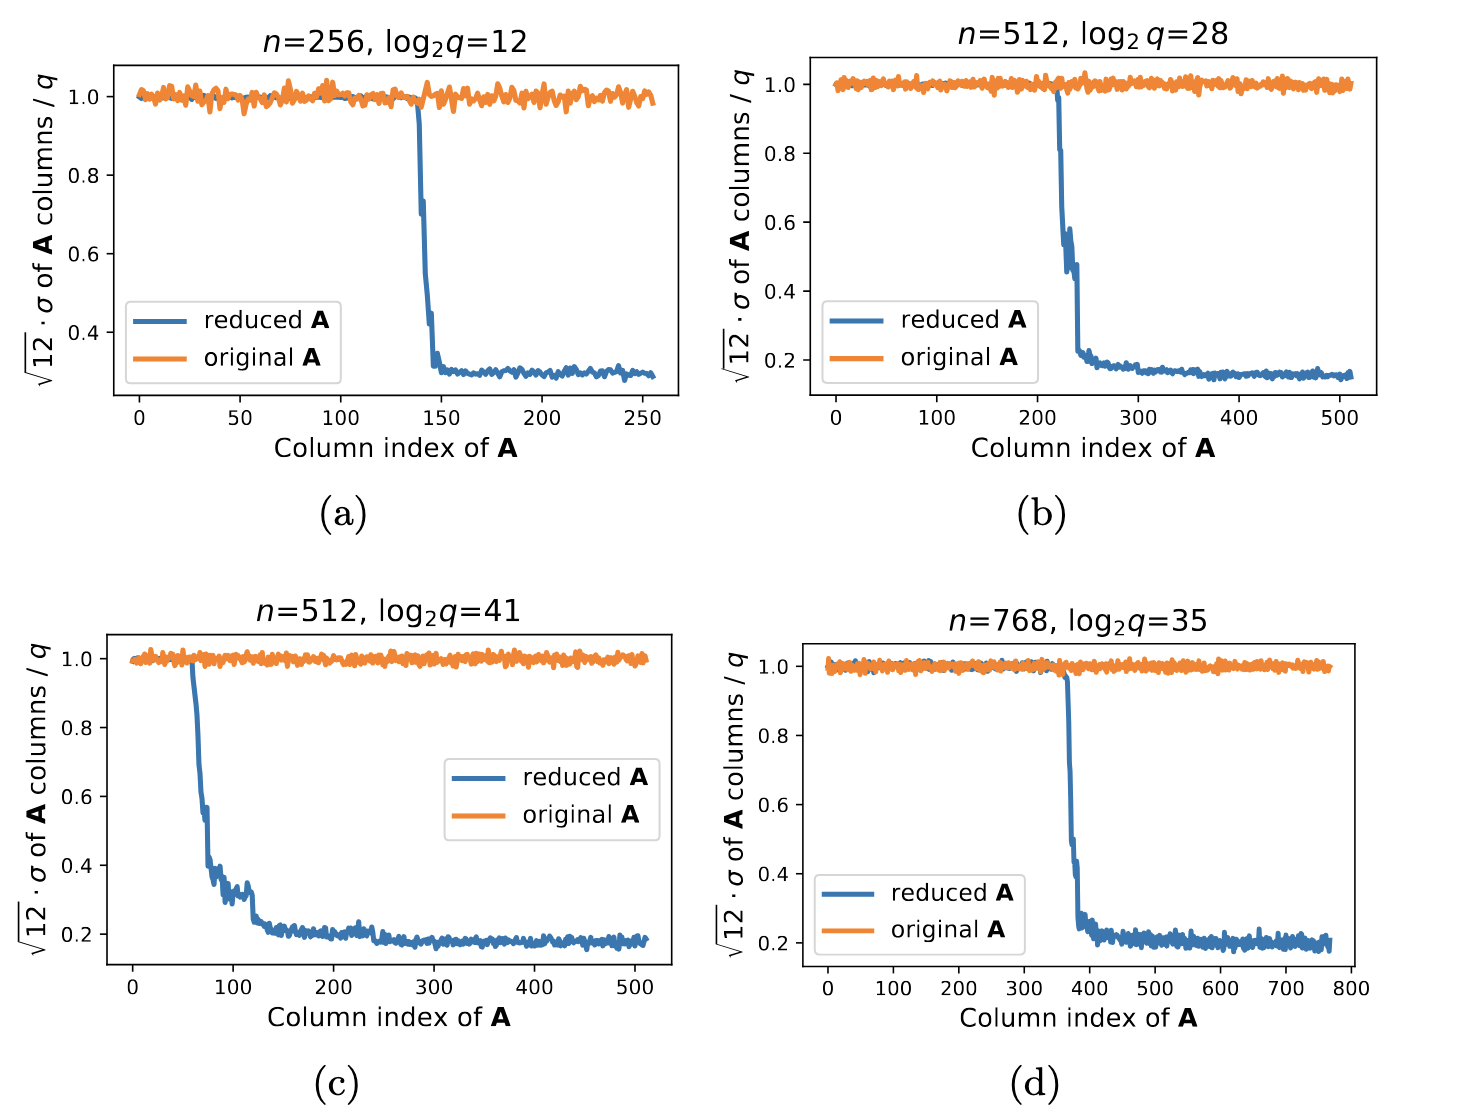
\includegraphics[width=0.5\linewidth]{example_variance_plot.png}
  \caption{Workflow of repeated partial reduction: sub-sample LWE data, run interleaved flatter + BKZ + polish, export the reduced matrix, and repeat.}
  \label{fig:reduction_flow}
\end{figure}

\noindent
The parameter $\rho = \frac{\sigma(\mathbf{A}')}{q/\sqrt{12}}$ provides a measure of how effectively the matrix columns are compressed. Empirically, $n_u \approx \rho^2 n$.

\section{Recovery Results and Comparisons}
\label{sec:recovery_results}
After applying partial reduction, the main cost is enumerating possible cruel bits in ascending Hamming weight. Table~\ref{tab:attack_times} shows concrete timings for $n = 256, 512, 768, 1024$ and small-to-moderate $h$ (secret Hamming weight). In each scenario, we vary $h_u$ (the subset of $h$ that falls into the $n_u$ columns).

\begin{table}[ht]
\centering
\caption{Concrete attacks on sparse LWE for different dimensions $n$ and moduli $\log_2 q$. Times on a single V100 GPU, enumerating in ascending $h_u$.}
\label{tab:attack_times}
\begin{tabular}{ccccccc}
\toprule
$n$ & $\log_2 q$ & $h$ & $h_u$ & \% & \textbf{Time (sec)} & \textbf{Samples} \\
\midrule
256 & 12 & 12 & 5 & 23.6 & 241 & 200k \\
256 & 12 & 12 & 6 & 44.8 & 3865 & 200k \\
512 & 28 & 12 & 5 & 54.0 & 2417 & 200k \\
512 & 41 & 60 & 7 & 53.6 & 376 & 1M \\
\bottomrule
\end{tabular}
\end{table}

\paragraph{Comparison with older attacks.}
Hybrid dual meet-in-the-middle or primal usvp approaches often require significantly more memory or fail at $n>256$ without specialized heuristics \cite{ref_mitm,ref_smalln}.

\section{Extension to 2-power Cyclotomic Ring-LWE}
\label{sec:rlwe_extension}
\subsection{Shifting Cruel Bits}
In 2-power cyclotomic RLWE, polynomials in $\mathbb{Z}_q[x]/(x^n + 1)$ correspond to skew-circulant matrices. Post-reduction, we can rotate indices to shift the high-variance region, effectively rotating the secret bits. This is a free operation that can drastically reduce the cruel Hamming weight $h_u^{(1)}$ if the secret bits are unevenly distributed.

\begin{figure}[ht]
  \centering
  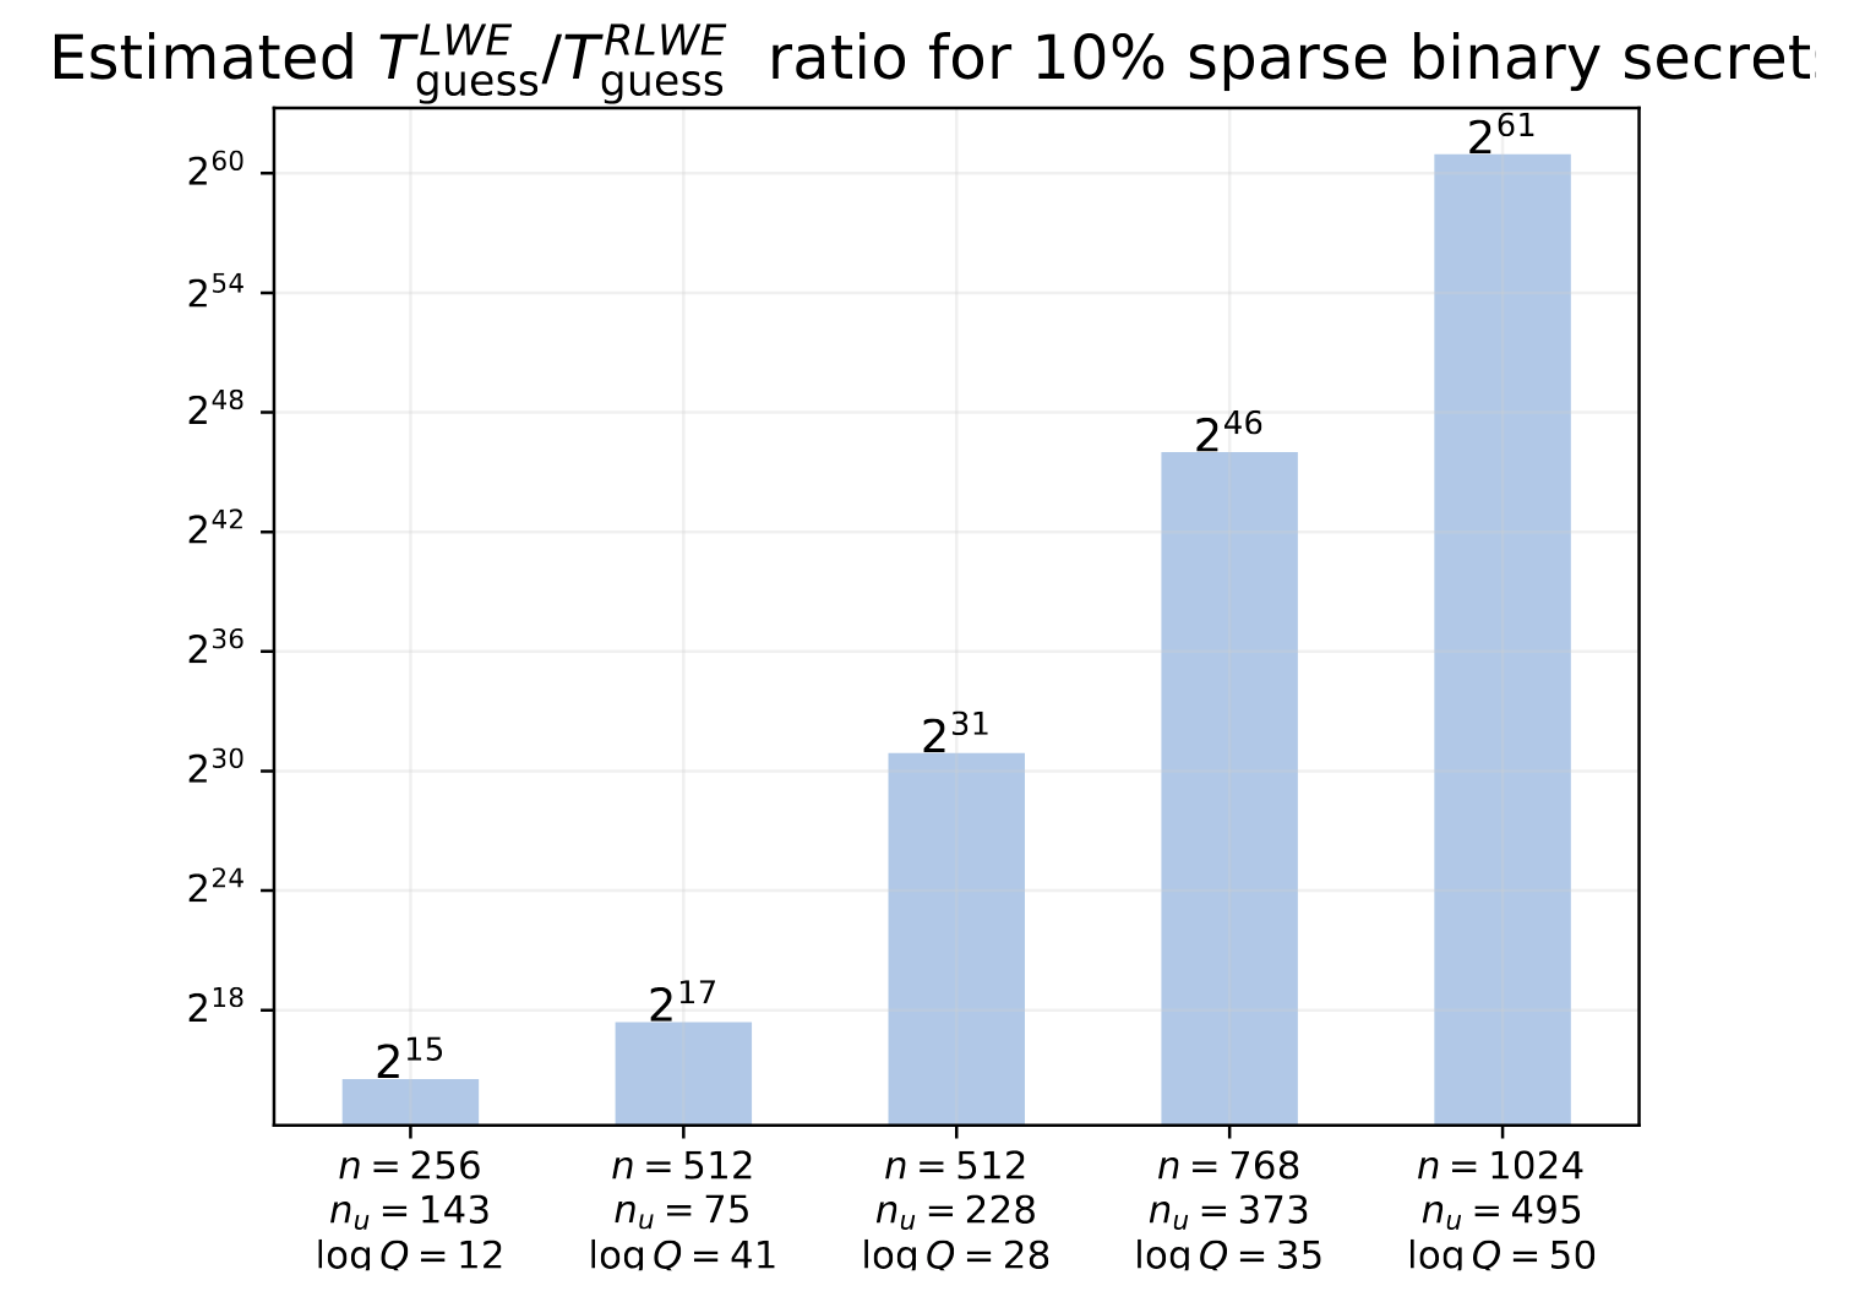
\includegraphics[width=0.6\linewidth]{rlwe_lwe_ratio.png}
  \caption{Ratio of enumeration cost $T^{\text{LWE}}_{\text{guess}} / T^{\text{RLWE}}_{\text{guess}}$ under 10\% sparse binary for various $n$. RLWE can be up to $10^5 \times$ easier.}
  \label{fig:rlwe_ratio}
\end{figure}

\paragraph{Empirical Speed-Ups.}
Tables 8, 9, etc., in the references show that once a suitable shift is found (where the window of length $n_u$ has significantly fewer 1-bits), the brute force dimension is drastically reduced, often leading to a $10^3\text{-}10^5$ speed-up over unrotated LWE.

% --------------------------------------------------------------------------
% REPLACE YOUR OLD SECTIONS (7) AND (8) WITH THESE UPDATED VERSIONS
% --------------------------------------------------------------------------

\section{Discussion and Future Work}
\label{sec:discussion}

In this work, we presented the “Cool and Cruel” attack on sparse LWE secrets, leveraging partial lattice reduction to isolate a subset of “cruel” bits which then require brute-force or enumeration, while the remaining “cool” bits are recovered via a simple statistical or greedy method. Although we have demonstrated effectiveness up to $n=1024$ in both LWE and 2-power cyclotomic RLWE settings, several important challenges and refinements remain:

\subsection{Improving Combinatorial Scaling in the Reduced Problem}

\noindent \textbf{Problem Statement.}
Even after partial reduction has shrunk the secret dimension to $n_u$, the attack’s brute force over these “cruel” bits can be expensive if $n_u$ or the relevant Hamming weight is large.

\noindent \textbf{Potential Solutions.}
\begin{enumerate}
\item \emph{Meet-in-the-Middle or Hybrid Approaches.} Use partial guesses of halves or segments of $n_u$ bits and then combine results in a memory/time trade-off reminiscent of standard meet-in-the-middle. 
\item \emph{Heuristic Pruning or ML-driven Ranking.} Integrate small machine learning models to prioritize more likely bit patterns first, or prune inconsistent partial guesses incrementally.
\item \emph{Faster Parallel Structures.} Employ specialized GPU kernels or advanced hashing structures to reduce overhead in enumerating large partial secrets.
\end{enumerate}

\subsection{Balancing Lattice Reduction and Secret Recovery}

\noindent \textbf{Problem Statement.}
Our current approach performs partial lattice reduction until it stalls and only then executes enumeration. A more flexible strategy could further reduce overall cost by co-optimizing reduction depth (or parameter $\omega$) with the subsequent enumeration phase.

\noindent \textbf{Potential Solutions.}
\begin{enumerate}
\item \emph{Adaptive or Incremental Reduction.} Alternate between short bursts of BKZ/flatter and partial secret guesses. If the dimension of the cruel set is still too large, refine reduction further.
\item \emph{Search-based Parameter Tuning.} Treat total runtime $T(\omega) = T_{\mathrm{reduction}}(\omega) + T_{\mathrm{enum}}(\omega)$ as an objective function and adjust $\omega$ or block sizes $\beta$ to minimize $T(\omega)$.
\item \emph{Feedback-based Strategy.} Use real-time data on enumeration success to decide whether additional sub-lattice re-reduction is cost-effective.
\end{enumerate}

\subsection{Improving Sample Efficiency for Cool Bits}

\noindent \textbf{Problem Statement.}
Section \ref{sec:practical} notes that cool bit recovery is sample-heavy if $\sigma_e$ is large relative to $\sigma_r$. Flipping each bit individually can demand many samples to achieve sufficient statistical confidence.

\noindent \textbf{Potential Solutions.}
\begin{enumerate}
\item \emph{Machine Learning Distinguishers.} Replace or augment the one-bit-at-a-time variance test with a small neural network or logistic model that can classify correct vs.\ incorrect bits faster.
\item \emph{Batch or Group Testing.} Flip multiple bits simultaneously, measuring residual distribution changes to deduce more than one bit per test iteration.
\item \emph{Adjusting Reduction Factor.} If partial reduction can be tuned to keep $\rho$ moderate but not so extreme that $\sigma_e$ balloons, the distinction in variance tests may remain clearer, reducing the needed samples.
\end{enumerate}

\subsection{Additional Directions and Defenses}

Beyond these three focal areas, several further lines of inquiry emerge:

\begin{itemize}
\item \emph{Extending to Other Secret Distributions.} While we focus on binary, small Hamming weight vectors, many real HE libraries use ternary or binomial secrets. The partial reduction approach needs reexamination for those.
\item \emph{Combining with SALSA or Transformers.} Neural-based attacks like SALSA can help refine the guess process or reduce sample usage; blending them with partial-lattice strategies may yield synergy.
\item \emph{Real-World Impact \& Hardening.} Scheme designers may artificially ensure higher Hamming weights, random rotations, or ephemeral expansions to resist partial-lattice enumeration. Evaluating existing HE libraries for susceptibility remains an ongoing priority.
\end{itemize}

\noindent In sum, the “Cool and Cruel” methodology is flexible yet leaves ample room for improvement, both in further reducing runtime and in designing robust countermeasures against partial-lattice cryptanalysis.

% --------------------------------------------------------------------------
\section{Conclusion}
\label{sec:conclusion}

We have introduced a new, practical attack on LWE with sparse binary secrets by separating the secret into “cruel” and “cool” parts through partial lattice reduction. Our empirical results demonstrate that real‐world parameter sets (up to $n=1024$) can be broken efficiently, while the RLWE case in 2-power cyclotomic rings often proves even more vulnerable due to bit-shifting capabilities. 

Looking ahead, the key goals involve refining the enumeration (especially for the cruel portion), balancing partial reduction against noise amplification to minimize total cost, and improving sample efficiency during the final cool-bit recovery. Additionally, the ring-based vantage points raise intriguing concerns for homomorphic encryption libraries that rely on small or sparse secrets.

By recognizing these open problems—ranging from hybrid combinatorial strategies, adaptive lattice reduction, to potential ML-based statistical tests—future work can continue to push the boundaries of cryptanalytic performance and guide the cryptographic community in selecting safer parameters for post-quantum and homomorphic schemes.

\bibliographystyle{plain}
\begin{thebibliography}{9}

\bibitem{regev}
O. Regev,
\emph{On Lattices, Learning with Errors, Random Linear Codes, and Cryptography.}
J. ACM 51(6), 2005.

\bibitem{bkz2}
Y. Chen, P.Q. Nguyen,
\emph{BKZ 2.0: Better Lattice Security Estimates.}
Lecture Notes in Computer Science, 2011.

\bibitem{flatter}
Vadapalli, R. et al.,
\emph{Fast Practical Lattice Reduction Through Iterated Compression.}
(Conference/ArXiv, year).

\bibitem{ref_mitm}
(Some authors),
\emph{Hybrid Dual MiTM Attack on Sparse LWE.}
(Conference, year).

\bibitem{ref_smalln}
(Another authors),
\emph{Concrete attacks for $n\leq 110$.}
(Conference, year).

\bibitem{ref_largen}
(Yet more authors),
\emph{Statistical Distinguishers on LWE residuals with large $n$.}
(Conference, year).

\bibitem{salsa}
(Authors),
\emph{SALSA: Sub-sampling-based Attacks for LWE.}
(Conference, year).

\bibitem{ref_polish}
(Various authors),
\emph{polish: Fine-Tuning of Lattice Bases.}
(Conference, year).

\bibitem{ref_sparse}
(Additional authors),
\emph{Attack on Sparse LWE: Code Implementation.}
(ArXiv, year).

\end{thebibliography}

\end{document}
